\documentclass{beamer}

\usepackage{geometry}
\usepackage{graphicx}
%\usepackage{wrapfig}
\usepackage{amsmath}

%\useoutertheme{infolines}
\usetheme{Boadilla}
\usecolortheme{seahorse}
\setbeamertemplate{navigation symbols}{}
\title{Computer Memory}
\newcommand{\shorttitle}{64 Bit Intel Assembly Language}
\newcommand{\shortauthor}{\copyright 2011 Ray Seyfarth}
\author{Ray Seyfarth}
\begin{document}


\usefoottemplate{\vbox{
\tinycolouredline{structure!55}%
 {\color{white}{\textbf{\shorttitle}\hfill\textbf{\shortauthor}}}%
}}

\begin{frame}
    \titlepage
\end{frame}
\begin{frame}
\frametitle{Outline}
\tableofcontents
\end{frame}

\section{Memory mapping}


\begin{frame}
    \frametitle{Memory mapping}
    \begin{itemize}
        \item Computer memory is an array of bytes from 0 to $n-1$
              where $n$ is the memory size
        \item Programs perceive ``logical'' addresses which
              are mapped to physical addresses
        \item 2 people can run a program starting at logical address
              {\tt 0x4004c8} while using different physical memory
        \item CPU translates logical addresses to physical during
              instruction execution
        \item The CPU translation can be just as fast as if the software
              used physical addresses
        \item The x86-64 CPUs can map pages of sizes 4096 bytes and 2
            megabytes
        \item Linux uses 2 MB pages for the kernel and 4 KB pages for
            programs
        \item Some recent CPUs support 1 GB pages
    \end{itemize}

\end{frame}

\begin{frame}
    \frametitle{Translating an address}
    \begin{itemize}
        \item Suppose an instruction references address {\tt 0x43215628}
        \item With 4 KB pages, the rightmost 12 bits are an offset
              into a page
        \item With {\tt 0x43215628} the page offset is {\tt 0x628}
        \item The page number is {\tt 0x43215}
        \item Let's assume that the computer is set up to translate 
              page {\tt 0x43215} to physical addresses {\tt 0x7893000} - {\tt 0x7893fff}
        \item Then address {\tt 0x43215628} is mapped to {\tt 0x7893628} 
    \end{itemize}
\end{frame}

\begin{frame}
    \frametitle{Benefits of memory mapping}
    \begin{itemize}
        \item User processes are protected from each other
        \begin{itemize}
            \item Your {\tt vi} process can't read my {\tt vi}'s data
            \item Your process can't write my data
        \end{itemize}
        \item The operating system is protected from malicious or errant code
        \item It is easy for the operating system to give processes contiguous
              chunks of ``logical'' memory
    \end{itemize}
\end{frame}

\begin{frame}
    \frametitle{Why study memory mapping?}
    \begin{itemize}
        \item If you write programs, the mapping is automatic
        \item We will not discuss instructions for changing mapping tables
        \item So what difference does it make?
        \item It helps explain page faults
        \begin{itemize}
            \item Suppose you allocate an array of 256 bytes at
                  logical address {\tt 0x45678200}
            \item Then all addresses from {\tt 0x45678000} to
                  {\tt 0x45678fff} are valid
            \item You can go well past the end of the array before
                  you can get a segmentation violation
        \end{itemize}
        \item Knowledge is power!
    \end{itemize}
\end{frame}

\section{Process memory model in Linux}
\begin{frame}
    \frametitle{Process memory model in Linux}
    \begin{columns}
        \begin{column}[l]{3.5in}
            \begin{itemize}
                \item A Linux process has 4 logical segments
                \begin{itemize}
                    \item text: machine instructions
                    \item data: static data initialized when the program starts
                    \item heap: data allocated by {\tt malloc} or {\tt new}
                    \item stack: run-time stack
                    \begin{itemize}
                        \item return addresses
                        \item some function parameters
                        \item local variables for functions
                        \item space for temporaries
                    \end{itemize}
                \end{itemize}
                \item In reality it is more complex
                \item 131TB is 47 bits of all 1's
                \item CPU could use 48 bit logical addresses
                \item Canonical addresses propagate bit 47 through 48-63 so Linux chose to use 47 bits to avoid the top stack address from appearing huge
            \end{itemize}
        \end{column}
        \begin{column}[r]{3in}
            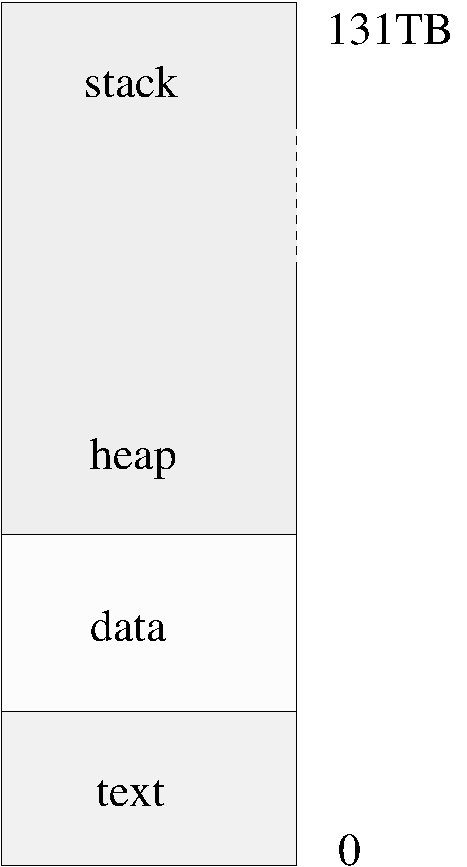
\includegraphics[width=1.5in]{process_memory.pdf}
        \end{column}
    \end{columns}
\end{frame}

\begin{frame}
    \frametitle{Memory segments}
    \begin{itemize}
        \item The text segment is named {\tt .text} in {\tt yasm}
        \begin{itemize}
            \item {\tt \_start} and {\tt main} are not actually at 0
            \item The text segment does not need to grow, so the data
                  segment can be placed immediately after it
        \end{itemize}
        \item The data segment is in 2 parts
        \begin{itemize}
            \item {\tt .data} which contains initialized data
            \item {\tt .bss} which contains reserved data (initialized to 0)
            \item ``bss'' stands for ``Block Started by Symbol''
        \end{itemize}
        \item The heap and the stack both need to grow
        \begin{itemize}
            \item The heap grows up
            \item The stack grows down
            \item They meet in the middle and explode
        \end{itemize}
        \item Use of heap and stack space in assembly does not involve
              using a named segment
    \end{itemize}
\end{frame}

\begin{frame}
    \frametitle{Stack segment limits}
    \begin{itemize}
        \item The stack segment is limited by the Linux kernel
        \item The typical size is 16 MB for 64 bit Linux
        \item This can be inspected using ``{\tt ulimit -a}''
        \item 16 MB seems fairly small, but it is fine until you start
              using large arrays as local variables in functions
        \item The stack address range is {\tt 0x7fffff000000} to {\tt 0x7fffffffffff}
        \item A fault to addresses in this range are recognized by the
            kernel to allow the stack to grow as needed
    \end{itemize}
\end{frame}

\begin{frame}
    \frametitle{A few adjustments to the memory model}
    \begin{itemize}
        \item It appears that the text segment starts at {\tt 0x400000} not 0
        \item Shared libraries map code and data into lots of addresses
        \item You can map shared memory regions into your programs
        \item Use ``{\tt cat /proc/\$\$/maps}'' to see your shell's map
        \begin{itemize}
            \item {\tt \$\$} is the shell's process id
        \end{itemize}
    \end{itemize}
\end{frame}

\section{Memory example}

\begin{frame}[fragile]
    \frametitle{Memory example source code}
\begin{verbatim}
        segment .data
a       dd      4
b       dd      4.4
c       times   10 dd 0
d       dw      1, 2
e       db      0xfb
f       db      "hello world", 0

        segment .bss
g       resd    1
h       resd    10
i       resb    100
\end{verbatim}
\end{frame}

\begin{frame}[fragile]
    \frametitle{Memory example source code (2)}
\begin{verbatim}
      segment .text
      global  main     ; let the linker know about main
main:
      push    rbp      ; set up a stack frame for main
      mov     rbp, rsp ; set rbp to point to the stack frame
      sub     rsp, 16  ; leave some room for local variables
                       ; leave rsp on a 16 byte boundary
      xor     eax, eax ; set rax to 0 for return value
      leave            ; undo the stack frame manipulations
      ret    
\end{verbatim}
\end{frame}

\begin{frame}[fragile]
    \frametitle{Memory example listing file}
\begin{verbatim}
 1                                 %line 1+1 memory.asm
 2                                 [section .data]
 3 00000000 04000000               a dd 4
 4 00000004 CDCC8C40               b dd 4.4
 5 00000008 00000000<rept>         c times 10 dd 0
 6 00000030 01000200               d dw 1, 2
 7 00000034 FB                     e db 0xfb
 8 00000035 68656C6C6F20776F72-    f db "hello world", 0
 9 00000035 6C6400             
\end{verbatim}
    \begin{itemize}
        \item Addresses are relative to start of {\tt .data} in this file
        \item Notice that the 4 byte of 4 is at address 0 (backwards)
        \item {\tt b} = {\tt 0x408ccccd} = {\tt 0 10000001 00011001100110011001101}
        \item Sign bit is 0, exponent field is {\tt 0x81} = 129, exponent = 2
        \item Fraction is {\tt 1.00011001100110011001101}
    \end{itemize}
\end{frame}

\begin{frame}[fragile]
    \frametitle{Memory example listing file (2)}
\begin{verbatim}
11                                 [section .bss]
12 00000000 <gap>                  g resd 1
13 00000004 <gap>                  h resd 10
14 0000002C <gap>                  i resb 100
\end{verbatim}
    \begin{itemize}
        \item Notice that the addresses start again at 0
        \item The commands reserve space
        \item {\tt resd 1} reserves 1 double word or 4 bytes
        \item {\tt resd 10} reserves 10 double words or 40 bytes
        \item {\tt resb 100} reserves 100 bytes
    \end{itemize}
\end{frame}

\begin{frame}[fragile]
    \frametitle{Memory example listing file (3)}
\begin{verbatim}
16                                 [section .text]
17                                 [global main]
18                                 main:
19 00000000 55                      push rbp
20 00000001 4889E5                  mov rbp, rsp
21 00000004 4883EC10                sub rsp, 16
22 00000008 31C0                    xor eax, eax
23 0000000A C9                      leave
24 0000000B C3                      ret
\end{verbatim}
\end{frame}

\section{Examining memory with {\tt gdb}}

\begin{frame}
    \frametitle{Examining memory with {\tt gdb}}
\begin{itemize}
    \item Time to try some commands in {\tt gdb}
    \item Use p for print
    \begin{itemize}
        \item Print allows printing expressions
        \item p/d for decimal
        \item try format options t, u, i, c, s, f, a and x
    \end{itemize}
    \item Examine requires a memory address
    \begin{itemize}
        \item x/NFS
        \item N is an optional count
        \item F is a format like print
        \item S is a size character: b=1, h=2, w=4, g=8
    \end{itemize}
\end{itemize}

\end{frame}

\section{Examining memory with {\tt ebe}}

\begin{frame}
    \frametitle{Examining memory with {\tt ebe}}
\begin{itemize}
    \item Run program to a breakpoint
    \item Control-right-click on a variable name
    \item Fill in popup form
    \begin{itemize}
        \item Variable name
        \item Address - will the {\tt \&variable}
        \item Format
        \begin{itemize}
              \item floating point
              \item decimal
              \item hexadecimal
              \item character
              \item string
              \item string array (like argv in main)
        \end{itemize}
        \item Size: 1, 2, 4 or 8 bytes
        \item First and last indices
    \end{itemize}
    \item Variable will be monitored in data window
\end{itemize}

\end{frame}
\end{document}
